% vim: expandtab softtabstop=2 shiftwidth=2 foldmethod=marker spell

\section{Importing Songs}
How to import songs from a CSV (Comma Separated Values) file.

A CSV file is literally its name, just a bunch of things separated by commas. Due to its very simple nature, CSV files can be edited with most programs including Wordpad, but common editors include Google Sheets and Microsoft Excell.

In the table below, you can see what an example of a comma separated values songlist would look like. 
The first line of the file names the columns, such as title, artist, and active. 

\begin{table}[h!]
\pgfplotstabletypeset[col sep=comma,
  string type,
  columns={title,artist,active},
  every head row/.style={before row=\hline,after row=\hline},
  every last row/.style={after row=\hline},
  every even row/.style={before row=\rowcolor[gray]{0.9}},
  every first column/.style={column type/.add={|}{}},
  every column/.style={column type/.add={}{|}},
  ]{src/songlist_import/example.csv}
\caption{Songlist Example CSV}
\label{example.csv}
\end{table}

Active is a bit special in that it uses a classical boolean value. 
A 0 represents that the song is off or inactive, and a 1 represents that song is on or active.
An inactive song can is no longer shown as part of the normal user songlist, but instead can be seen by mods and above in edit mode. 
When importing songs, it is best practice to have them as inactive, so that normal users are not able to use them until you are sure they are imported correctly, just in case something were to go wrong.
Inactive songs will be displayed in red when the "show inactive" slider is active.

\begin{figure}[ht!]
  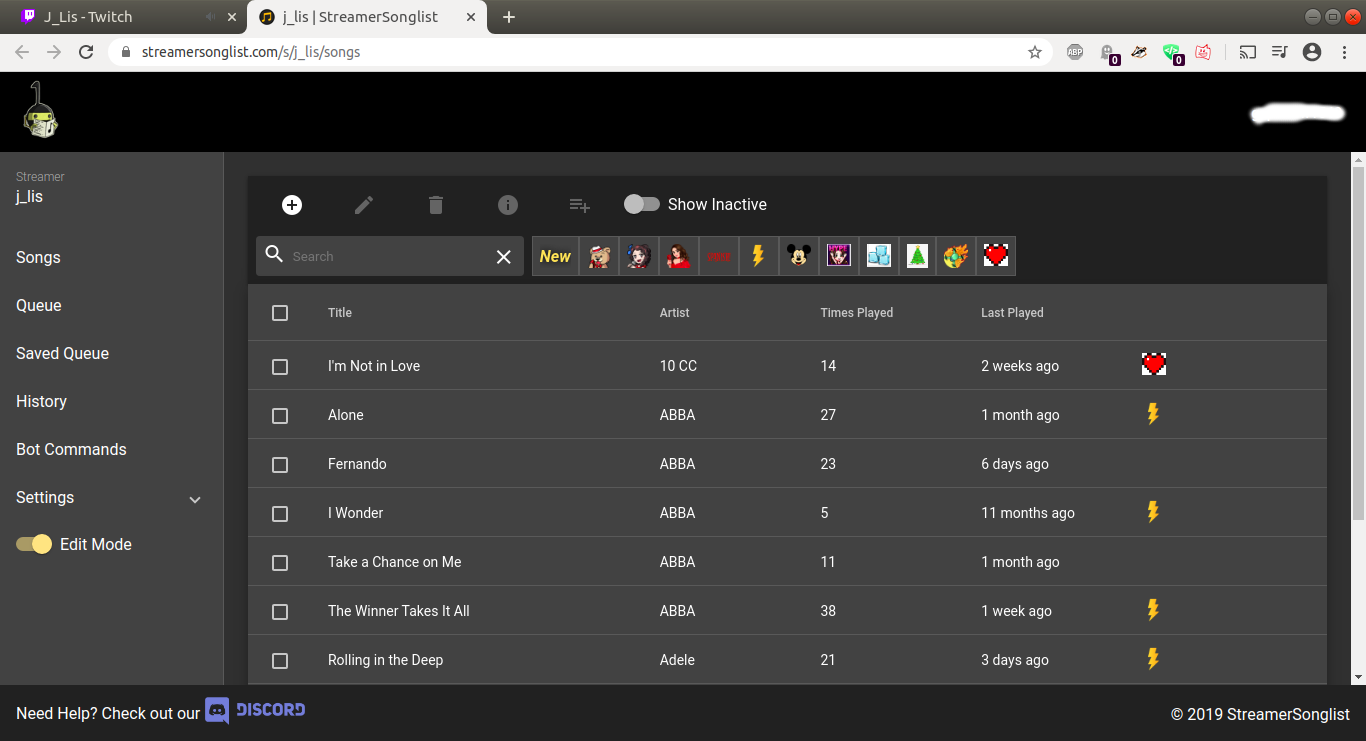
\includegraphics[width=\linewidth]{src/songlist_import/songlist_main_edit.png}
  \caption{The ``show inactive" slider}
  \label{show inactive}
\end{figure}

\begin{figure}[ht!]
  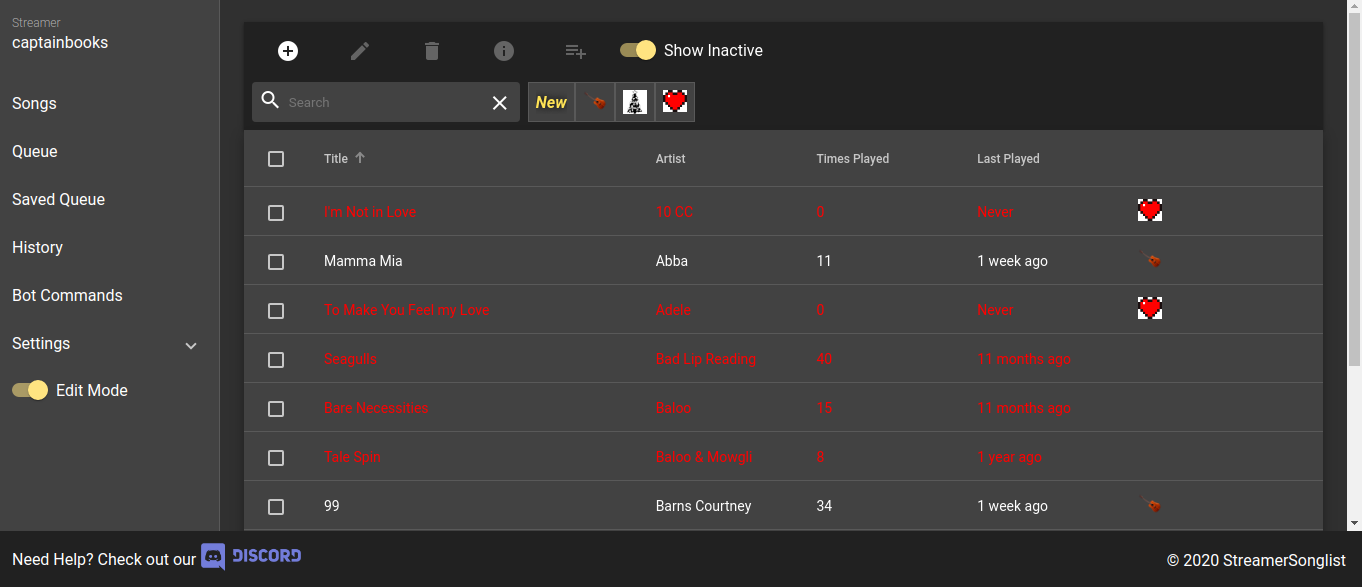
\includegraphics[width=\linewidth]{src/songlist_import/inactive_songs_displayed.png}
  \caption{The ``show inactive" slider activated}
  \label{acitve show inactive}
\end{figure}

\clearpage

Once your songlist is created as a CSV, you can add it from the import songs page.

\begin{figure}[ht!]
  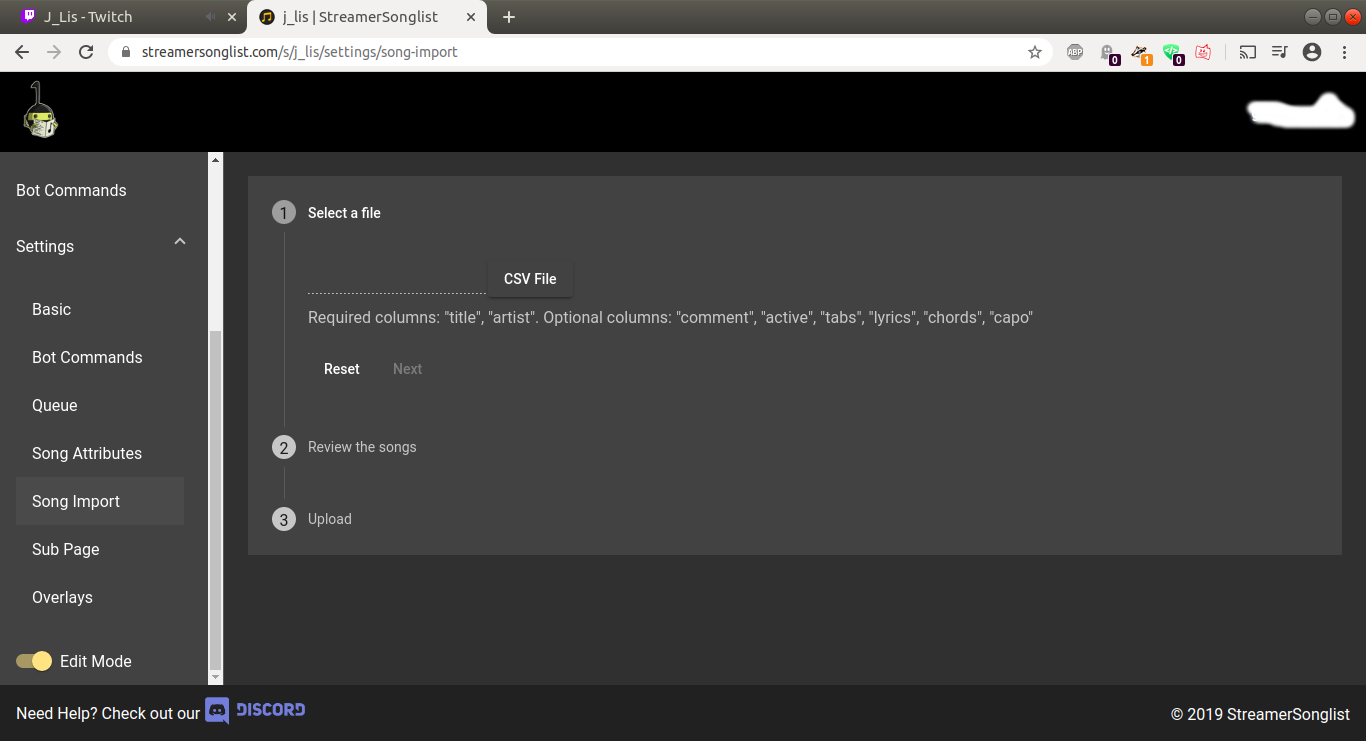
\includegraphics[width=\linewidth]{src/songlist_import/import_songs.png}
  \caption{The import songs page}
  \label{import songs}
\end{figure}
